\section{Modellazione end-effector}
L'obiettivo di questo capito consiste nel presentare la modellazione della cinematica e dinamica dell'end-effector.
\\L'end-effector, identificato anche come utensile, è composto da due parti: 
\begin{figure}[ht]
	\begin{center}
		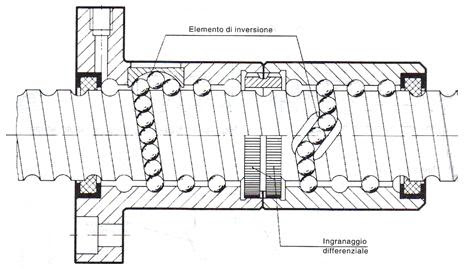
\includegraphics[scale=0.5]{Immagini/ViteRicircolo}
		\caption{Struttura vite}
	\end{center}
\end{figure}
La prima è una vite a ricircolo di sfere che permette un movimento rotativo, mentre la seconda parte è una guida lineare che permette una traslazione positiva o negativa nell'asse z. Entrambi i componenti sono collegati a motori che permettono la movimentazione interfacciandosi con degli azionamenti. All'estermità della vite è possibile collegare un utensile, come è possibile vedere dalla foto è stato collegato un utensile utilizzato per disegnare le traiettorie su di un foglio.
\begin{figure}[ht]
	\begin{center}
		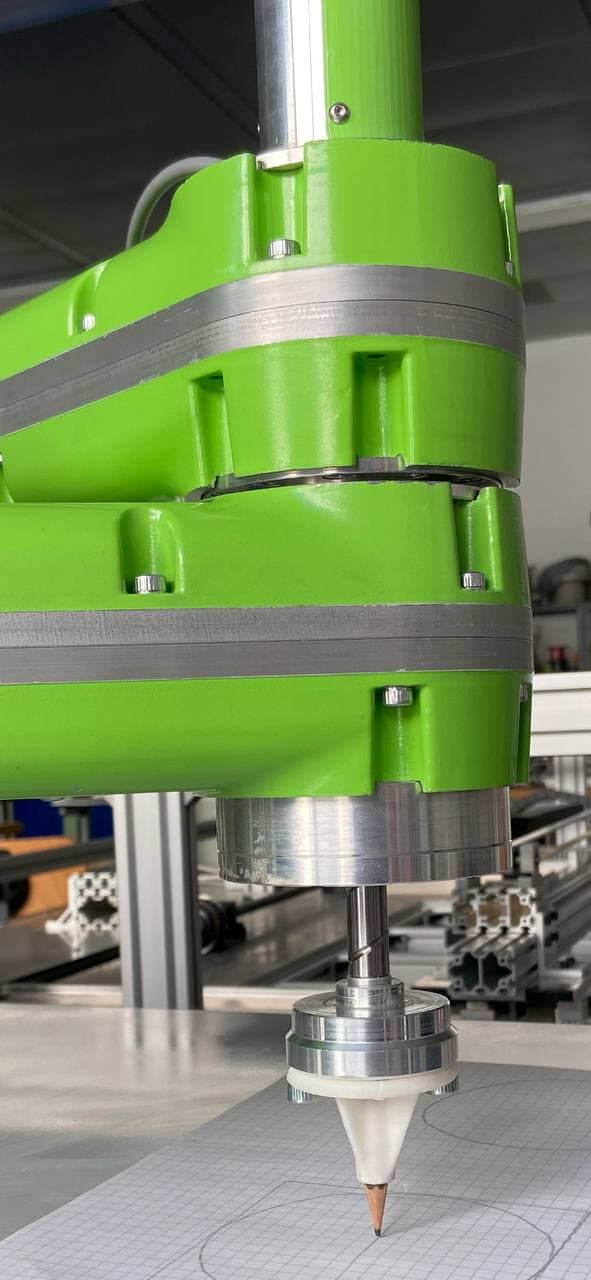
\includegraphics[scale=0.25]{Immagini/utensile}
		\caption{Utensile da disegno}
	\end{center}
\end{figure}
\\Per proseguire con la trattazione della parte cinematica e dinamica andiamo ad introdurre i parametri della vite:
\begin{table}[h!]
\centering
\begin{tabular}{|c |c |c|} 
 \hline
 Nome & Descrizione  & Valore \\ [0.5ex] 
 \hline\hline
 $m_v [kg]$ & massa vite  & 0.36 \\ 
 $p_v [m]$ & passo vite & 0.02 \\
 $I_v [kg\cdot m^2]$ & momento inerzia vite  & $6.40\cdot 10^{-6}$ \\
 \hline
\end{tabular}
\caption{Parametri end-effector}
\label{table:2}
\end{table}
\\A livello teorico si è partito definendo una legge di modo per entrambi i componenti della vite, si è selezionata una legge polinomiale, per la guida è stata fatta una legge sulla posizione, mentre per la vite a ricircolo di sfere sull'orientamento.
\subsection{Cinematica end-effector}
Come anticipato, abbiamo quindi la presenza di due leggi di moto che identifichiamo con $z_{ee}$ e $\varphi_v$. Il risultato della cinematica di posizione è il parametro V, per velocità ed accelerazione saranno le sue derivate, $\dot{V}$ e $\ddot{V}$ definite come: 
\begin{equation*}
	V = 
	\begin{bmatrix}
		Z \\ 
		\theta_Z
	\end{bmatrix}, 
	\dot{V} = 
	\begin{bmatrix}
		\dot{Z} \\ \dot{\theta_Z}
	\end{bmatrix},
	\ddot{V} =
	\begin{bmatrix}
		\ddot{Z} \\ \ddot{\theta_Z}
	\end{bmatrix}
\end{equation*}
V è composto da una parte di traslazione (Z) e da una parte di rotazione $\theta_Z$; Per andar a ricavare la cinematica abbiamo quindi bisogno della legge di moto e della jacobiana della vite, che possiamo definire come:
\begin{equation}
J_e =
    \begin{bmatrix}
    \frac{p_v}{2 \pi} & \frac{p_v}{2 \pi} \\
    0 & 1
    \end{bmatrix}
\end{equation}
Andando ora a combinare i parametri e sostituendoli nell'equazione precedente otteniamo:
\begin{equation}
    V = J_e \begin{bmatrix}
    z_{ee} \\ \varphi_v
    \end{bmatrix},
    \dot{V} = J_e \begin{bmatrix}
    \dot{z_{ee}} \\ \dot{\varphi_v}
    \end{bmatrix},
    \ddot{V} = J_e \begin{bmatrix}
    \ddot{z_{ee}} \\ \ddot{\varphi_v}
    \end{bmatrix}
\end{equation}

\subsection{Dinamica della vite}
Per la definizione della dinamica della vite è stata usata, come per la dinamica dei link la tecnica del PLV. Per questa soluzione avremo bisogno delle accelerazioni dei due elementi quindi $\ddot{Z_{ee}}$ e $\ddot{\varphi_v}$. Andiamo poi ad introdurre la matrice di massa della vite, composta dalla massa e dall'inerzia e definita come:
\begin{equation}
	M_v\begin{bmatrix}
	m_e & 0 \\ 0 & I_v
	\end{bmatrix}
\end{equation} 
La soluzione della dinamica la troviamo quindi come:
\begin{equation}
    C_{ee} = M_v
    J_e \begin{bmatrix}
    \ddot{z_{ee}} \\ \ddot{\varphi_v}
    \end{bmatrix}
\end{equation}
Sono poi stati eseguiti vari test per la movimentazione della vite a livello teorico, nella seguente immagine è possibile vedere un risultato di questi test, in particolare nella figura sono mostrate le coppie fornite ai motori della vite e la posizione iniziale e finale della vite, tutto questo in funzione del tempo.
\begin{figure}[ht]
\begin{center}
    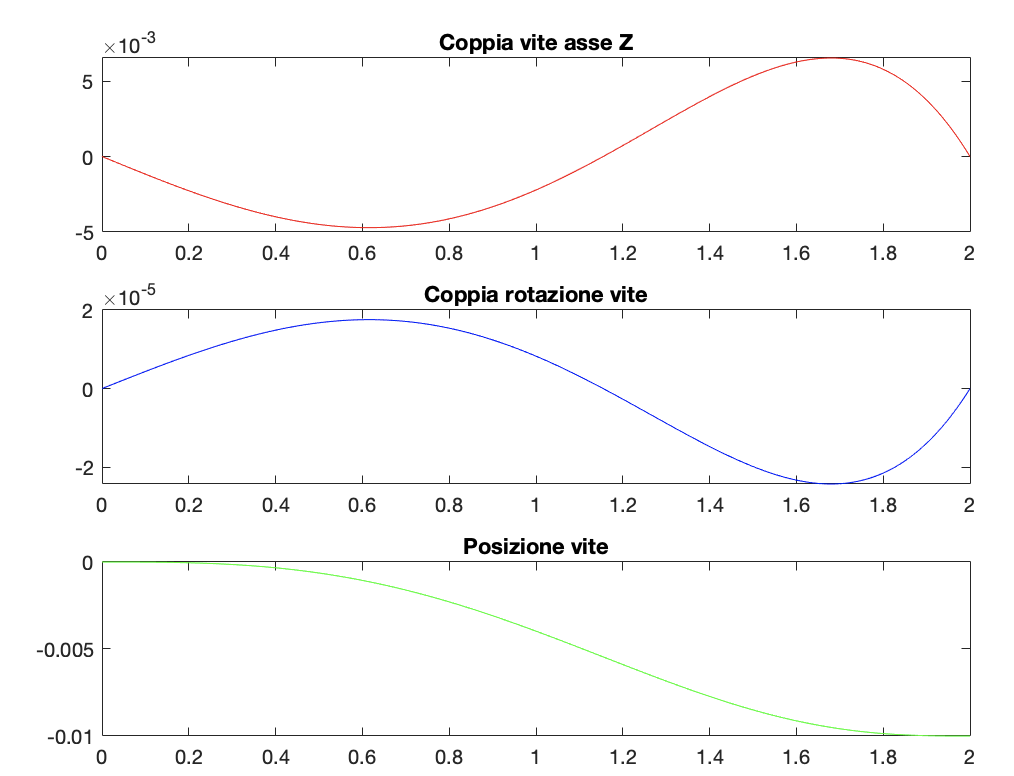
\includegraphics[scale=0.65]{Immagini/coppiaTeoricaVite.png}
    \caption{Coppie e posizione end-effector}
\end{center}
\end{figure}
